\documentclass[margin = 10pt]{standalone}
\usepackage{xcolor}
\usepackage{tikz}
\usepackage{pgfplots}
\pgfplotsset{
compat = 1.18
}
\pgfplotsset{
/pgfplots/colormap={cold}{
rgb255=(0,0,0) 
rgb255=(0,0,255) 
rgb255=(0,255,255)
rgb255=(255,255,255)
}
}
\begin{document}
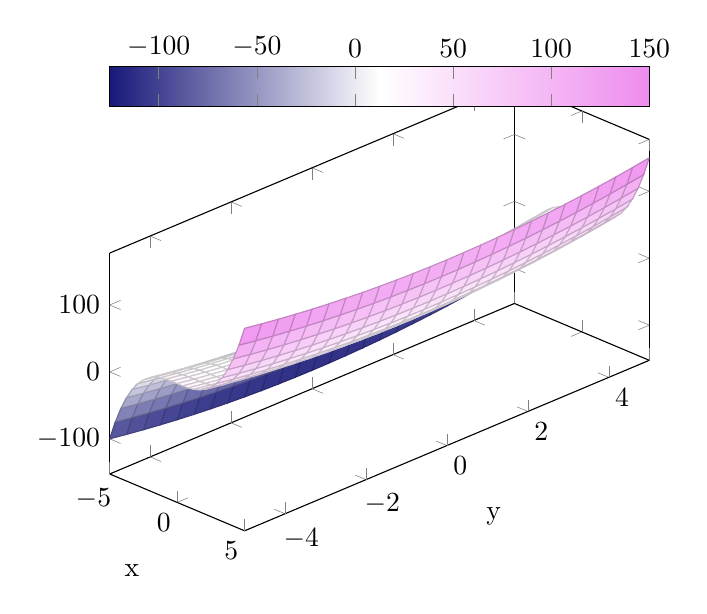
\begin{tikzpicture}
\begin{axis}[
    name = plot,
    plot box ratio=1 3 1,
    % 3D 图 或热力图相关
    % colorbar: horizontal | left | right 
    colorbar horizontal, % 必须配合算子参数 scatter or mesh 使用
    % blackwhite | greenyellow | violet | PuBu-9  (see pgf_plots.pdf, P420)
    colormap/violet,
    % colorbar/width=3mm,
    colorbar style={
        at = {(plot.north) },
        anchor = south,
        % right | left | upper | lower
        ticklabel pos= right,
        y dir=reverse
    },
    view={45}{20},
    surf,
    xlabel = x,
    ylabel = y,    
    ]
    
    
\addplot3 [
    surf,
    % mesh
] {x^3+y^2};
 
\end{axis}
\end{tikzpicture}
\end{document}